\documentclass[12pt]{article}
\usepackage{graphicx}
\usepackage{latexsym, amsmath,amsfonts,amssymb}
\usepackage{xcolor}
\usepackage{fancyhdr}
\usepackage{fancybox}
\usepackage{nccmath}%to get small medium and large math
\usepackage{natbib,todonotes}
\usepackage{wrapfig}
\usepackage[margin=1in]{geometry}
\usepackage{kpfonts}  %Changing the default fonts
\usepackage[T1]{fontenc}
\usepackage{tkz-euclide}
\setlength{\parskip}{1.2ex} %space between paragraphs
\setlength{\parindent}{1em} %Paragraph indentation
\clubpenalty = 10000
\widowpenalty = 10000
\newcommand\T{\rule{0pt}{2ex}} % \T will create extra space above (used to fix tables)
\newcommand\B{\rule[-1.5ex]{0pt}{0pt}}% \B will create extra space below (used to fix tables)
\usetikzlibrary{calc,trees,positioning,arrows,chains,shapes.geometric,%
  decorations.pathreplacing,decorations.pathmorphing,shapes,%
  matrix,shapes.symbols,plotmarks,decorations.markings,shadows}
\linespread{1.25} %spacing between lines
\newtheorem{Theorem}{Theorem}
\pagestyle{empty}
\begin{document}
\begin{center}
\Large{\textbf{Thales' Theorem (1)}}
\end{center}
\textbf{Thales' Theorem:} If $A$, $B$, and $C$ are points on a circle and
$\overline{AB}$ is a diameter of the circle then $\angle \,ACB$ is a right angle.\\

\begin{center}
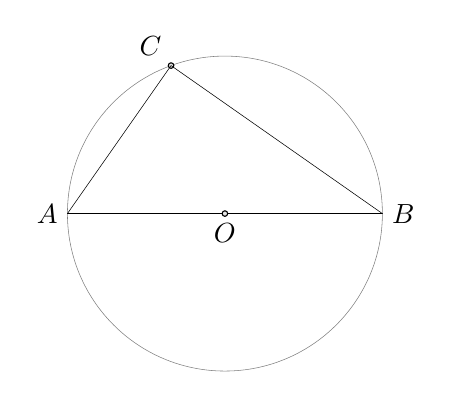
\begin{tikzpicture}[scale=2]
\tkzInit[xmin=-1.2,xmax=1.2,ymin=-1.2,ymax=1.2]
\tkzDefPoint(0,0){O}
\tkzDefPoint(1,0){B}
\tkzDefPoint(-1,0){A}
\tkzDrawCircle(O,A)
\tkzDrawSegment(A,B)
\tkzDefPoint(110:1){C}
\tkzDrawPoints(C,O)
\tkzDrawSegment(A,C)
\tkzDrawSegment(C,B)
\tkzLabelPoints[right](B)
\tkzLabelPoints[above left](C)
\tkzLabelPoints[left](A)
\tkzLabelPoints[below](O)
\end{tikzpicture}
\end{center}

\noindent \textbf{Proof:} Start by drawing the line segment $\overline{OC}$; this
breaks up the original triangle into two smaller triangles $ACO$ and $OCB$. Since $C$ is on 
the circle, both $ACO$ and $OCB$ are isosceles triangles. This means that in triangle $ACO$ 
angles $OAC$ and $OCA$ are the base angles. These base angles must be equal, so label them
$\alpha$. Likewise, triangle $OCB$ is a right triangle with base angles $OCB$ and $OBC$. Label
those angles $\beta$. This is illustrated in the next diagram. 
\begin{center}
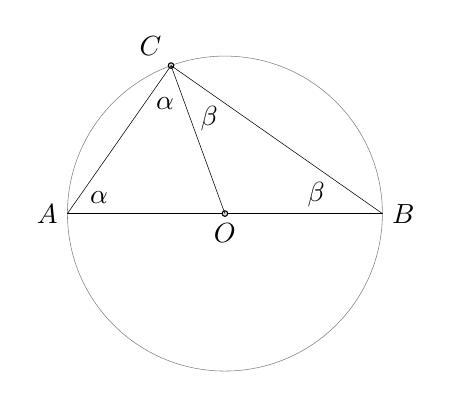
\begin{tikzpicture}[scale=2]
\tkzInit[xmin=-1.2,xmax=1.2,ymin=-1.2,ymax=1.2]
\tkzDefPoint(0,0){O}
\tkzDefPoint(1,0){B}
\tkzDefPoint(-1,0){A}
\tkzDrawCircle(O,A)
\tkzDrawSegment(A,B)
\tkzDefPoint(110:1){C}
\tkzDrawPoints(C,O)
\tkzDrawSegment(A,C)
\tkzDrawSegment(C,B)
\tkzDrawSegment(C,O)
\tkzLabelPoints[right](B)
\tkzLabelPoints[above left](C)
\tkzLabelPoints[left](A)
\tkzLabelPoints[below](O)
\tkzText(-.8,.1){$\alpha$}
\tkzText(-.38,.7){$\alpha$}
\tkzText(-.10,.6){$\beta$}
\tkzText(.58,.12){$\beta$}
\end{tikzpicture}
\end{center}

By the Triangle Sum Theorem, $\alpha + (\alpha + \beta) + \beta = 180^{\circ}$ which 
simplifies to $2\alpha + 2\beta = 180^{\circ}$ or, equivalently, $\alpha + \beta = 90^{\circ}$.
This implies $\angle \,ACB$ is a right angle and $\triangle \,ACB$ is a right triangle. Since
$C$ is an arbitrary point, Thales' Theorem has been proven.
\end{document}